\section{Odvození rovnic jednobodové kinetiky}

Pro odvození se vychází z 1G difúzní rovnice (s konstantním $D$ a $\Sigma_a$):

\begin{equation}
  \boxed{
  \dfrac{\partial n(\textbf{r}, t)}{\partial t} = D \Delta \Phi (\textbf{r}, t) - \Sigma_a \Phi (\textbf{r}, t) + Q (\textbf{r}, t),
  \label{difuzka}}
\end{equation}

kde:

\begin{itemize}
  \item $n$ (1/cm$^3$) značí hustotu neutronů,
  \item $D$ (cm) značí difúzní koeficient,
  \item $\Phi$ (1/cm$^2$s) značí hustotu toku neutronů,
  \item $\Sigma_a$ (1/cm) značí makroskopický účinný průřez pro absorbci a
  \item $Q$ (1/cm$^3$s) značí zdroj neutronů.
\end{itemize}

\subsection{Odvození bez vlivu zpožděných neutronů}

Uvažuji zjednodušení tvaru:

$$ Q (\textbf{r}, t) = k_\infty \Sigma_a \Phi (\textbf{r}, t), $$

$$ L^2 = \dfrac{D}{\Sigma_a}, $$

$$ B_m^2 = \dfrac{k_\infty - 1}{L^2}, $$

$$ n(\textbf{r}, t) = \dfrac{\Phi (\textbf{r}, t)}{v}$$

kde:

\begin{itemize}
  \item $k_\infty$ (-) značí koeficient násobenní pro nekonečný systém,
  \item $L$ (cm) značí difúzní délku (po umocnění difúzní plochu),
  \item $B_m$ (1/cm) značí materiálový faktor a
  \item $v$ (cm/s) značí rychlost neutronů (je konstantní, jelikož máme 1G přiblížení)
\end{itemize}

a předpokládáme, že rovnici \eqref{difuzka} lze řešit metodou separace proměnných, tedy:

$$ \Phi (\textbf{r}, t) = \Psi (\textbf{r}) \cdot T(t). $$

Poté rovnice \eqref{difuzka} vede na rovnici:

\begin{equation}
  v D \left ( \dfrac{\Delta \Psi (\textbf{r})}{\Psi (\textbf{r})} + B_m^2 \right ) = \dfrac{1}{T(t)} \dfrac{d T(t)}{d t} = \text{konst.} = - \omega,
  \label{difuzka_v_separaci}
\end{equation}

tedy na 2 obyčejné diferenciální rovnice provázané konstantou $\omega$.\\

Rovnice s $\Psi (\textbf{r})$ vede po uvažování okrajových podmínek (extrapolované rozhraní, konečnost, spojitost apod.) na vlastní funkce, jejichž tvar závisí na použité geometrii a tvaru Laplaciánu (kombinace goniometrických, Besselových, hyperbolických apod.). Řešení vyplývá z jednoduché vlnové rovnice:

$$ \Delta \Psi (\textbf{r}) + B_n^2 \Psi (\textbf{r}) = 0, $$

kde vztah mezi \textbf{vlastními čísly} $B_n$ a \textbf{materiálovým faktorem} $B_m$ je svázán pomocí určené konstanty $\omega$ jako:

$$ \omega_n = vD \cdot (B_n^2-B_m^2). $$

Obecně lze výsledek zapsat tvarem:

$$ \Psi (\textbf{r}) = \sum_n A_n \Psi_n (\textbf{r}), $$

kde $A_n$ značí normalizační konstantu a zjistíme ji z výkonu reaktoru.\\

Rovnice s $T(t)$ vede na exponenciálu tvaru:

$$ T(t) = C e^{- \omega t}. $$

Jelikož je ovšem $\omega$ závislá na volbě vlastních čísel, tak i zde platí superpozice a celkovou hustotu toku neutronů $\Phi (\textbf{r}, t)$ spočteme přes sumu všech vlastních funkcí jako:

\begin{equation}
  \Phi (\textbf{r}, t) = \sum_n A_n \Psi_n (\textbf{r}) e^{- \omega_n t}.
  \label{difuzka_reseni}
\end{equation}

Tabulka \ref{table_vlastni_funkce} udává vlastní čísla a vlastní funkce pro různé geometrie reaktoru (viz ZAF2).

\begin{table}[H]
\centering
\caption{Vlastní čísla a vlastní funkce pro různé geometrie.}
\label{table_vlastni_funkce}
\begin{tabular}{@{}rcc@{}}
\toprule
\textbf{Geometrie}   & $B_n$ (1/cm)         & $\Psi_n$ (-)                               \\ \midrule
\textbf{Nek. deska}  & $n \left ( \dfrac{\pi}{a} \right )$   & $\cos(B_nx)$              \\ [15pt]
\textbf{Nek. válec}  & $n \left ( \dfrac{2,405}{R} \right )$ & $J_0(B_nr)$               \\ [15pt]
\textbf{Koule}       & $n \left ( \dfrac{\pi}{R} \right )$   & $\dfrac{\sin(B_nr)}{r}$   \\ \bottomrule
\end{tabular}
\end{table}

Jelikož vlastní čísla splňují bilanci $B_1 < B_2 < B_3 < ...$, platí to samé i pro $\omega_1 < \omega_2 < \omega_3 < ...$ a první vlastní číslo po chvíli převáží ta zbylá. Proto dále zavádíme \textbf{geometrický faktor} $B_g$ jako první nejmenší vlastní číslo, tedy $B_g = B_1$.\\

Pro stacionární systém navíc platí $\omega = 0$ a poté $B_m = B_g$ (viz ZAF2).\\

Nyní přejdeme k prostorové nezávislosti (což je vlastně smysl celé kapitoly :D). Lze uvažovat (za předpokladu převážení prvního členu v rovnici \eqref{difuzka_reseni}), že:

$$ \Phi (\textbf{r}, t) \doteq v n(t) \Psi_1 (\textbf{r}) $$

a hustota neutronů $n(t)$ je zároveň úměrná maximální hustotě toku v soustavě (předpoklad rovnice jednobodové kinetiky), tedy:

$$ n(t) \doteq \text{konst.} \cdot \Phi_{max} (t). $$

Po dosazení do rovnice \eqref{difuzka_v_separaci} získáme novou rovnici tvaru:

\begin{equation}
  v D \left ( \dfrac{\Delta \Psi_1 (\textbf{r})}{\Psi_1 (\textbf{r})} + B_m^2 \right ) = \dfrac{1}{n(t)} \dfrac{d n(t)}{d t} = \text{konst.} = - \omega_1,
  \label{rovnice_kinetiky_v_separaci}
\end{equation}

která opět vede na 2 obyčejné diferenciální rovnice provázané konstantou $\omega_1$. Nyní už ovšem nejde o superpozici, jelikož uvažujeme pouze první člen (ačkoliv nestacionaritu zachováváme).\\

Pro zopakování a osvěžení paměti, stále platí:

$$ B_g = B_1, $$

$$ \omega_1 = vD \cdot (B_g^2 - B_m^2). $$

Zavedeme novou veličinu $\ell$ (s) jako \textbf{střední dobu života neutronů} vztahem:

\begin{equation}
  \boxed{
  \ell \equiv \dfrac{1}{v \Sigma_a} \dfrac{1}{1+L^2B_g^2}
  \label{stredni_doba_zivota}}
\end{equation}

a připomeneme si 1G rovnici pro stacionární reaktor:

$$ k_{\text{ef}} = \dfrac{k_{\infty}}{1 + L^2 B_g^2}. $$

Z těchto dvou vztahů lze vyjádřit parametr $\omega_1$ (důkaz dosazením) jako:

$$ \omega_1 = -\dfrac{k_{\text{ef}} - 1}{\ell}, $$

Což lze dosadit do rovnice \eqref{rovnice_kinetiky_v_separaci} (část s $\Psi$ už nemusím řešit) a získáváme \textbf{Rovnici jednobodové kinetiky}:

\begin{equation}
  \boxed{
  \dfrac{dn(t)}{dt} = \dfrac{k_{\text{ef}} - 1}{\ell} n(t).
  \label{rovnice_kinetiky_reseni}}
\end{equation}

Tím jsme si odvodili obyčejnou diferenciální rovnici 1. řádu pro hustotu neutronů $n(t)$, kterou lze řešit jednoduše pomocí integračního faktoru/separace proměnných (čímkoliv). Často nás ale více než hustota neutronů zajímá časový vývoj výkonu, tedy $P(t)$. Zde platí jednoduchá úměra:

$$ n(t) \sim P(t) $$

a tedy po přenormování platí:

$$ \dfrac{dP(t)}{dt} = \dfrac{k_{\text{ef}} - 1}{\ell} P(t). $$

S předpokladem počáteční podmínky $P(0) = P_0$ a úvahy, že $k_{\text{ef}} = \text{konst.}$, poté rovnice jednobodové kinetiky pro výkon dává řešení tvaru:

\begin{equation}
  P(t) = P_0 \exp \left ( \dfrac{k_{\text{ef}} - 1}{\ell} t \right ).
  \label{rovnice_kinetiky_vykon}
\end{equation}

\small

\textbf{Př. 1 -- perioda reaktoru:}

Rovnice \eqref{rovnice_kinetiky_vykon} udává, jak rychle se mění výkon v systému v závislosti na $k_{\text{ef}}$ a $\ell$. Zadefinujeme si \textbf{periodu reaktoru} $T_e$ (s) jako dobu, za kterou se výkon v systému změní e-krát, pomocí vztahu:

\begin{equation}
  \boxed{
  T_e \equiv \dfrac{\ell}{k_{\text{ef}} - 1}.
  \label{perioda}}
\end{equation}

Zatímco $k_{\text{ef}}$ lze ovlivnit (geometrie, obohacení, materiály), $\ell$ je pevně dáno a spjato se systémem\footnote{Teoreticky to lze také ovlivnit, ale asi těžko z rychlého reaktoru udělám tak jednoduše lehkovodní, žejo.}. Přehled rozsahů pro různé systémy zobrazuje tabulka \ref{table_stredni_doby_zivota}. Je tedy vidět, že např. rychlý reaktor bude na změny $k_{\text{ef}}$ reagovat mnohem rychleji, než reaktor moderovaný grafitem.\\

\begin{table}[H]
\small
\centering
\caption{\small Střední doby života pro různé typy reaktorů.}
\label{table_stredni_doby_zivota}
\begin{tabular}{@{}rc@{}}
\toprule
\textbf{Typ systému} & $\ell$ (s)           \\ \midrule
\textbf{FR}          & $10^{-7}$            \\
\textbf{LWR}         & $10^{-5} - 10^{-4}$  \\
\textbf{Grafit}      & $10^{-3}$            \\ \bottomrule
\end{tabular}
\end{table}

Pokud uvažujeme LWR reaktor ($\ell = 10^{-5}$), tak pro:

\begin{itemize}
  \item $k_{\text{ef}} = 1,01$ vychází perioda $T_e = 0,01$~s a za 1~s se změní výkon $2,69 \cdot 10^{43}$x,
  \item $k_{\text{ef}} = 1,001$ vychází perioda $T_e = 0,1$~s a za 1~s se změní výkon $2,20 \cdot 10^{4}$x,
  \item $k_{\text{ef}} = 1,0001$ vychází perioda $T_e = 1$~s a za 1~s se změní výkon $2,72$x.
\end{itemize}

\normalsize

K rovnici \eqref{rovnice_kinetiky_reseni} je možné dojít i jednoduchou úvahou. Jelikož platí úměra mezi $n(t)$ a $N(t)$:

$$ n(t) \sim N(t), $$

lze vycházet právě z počtu neutronů v jedné generaci. Pro přírůstek mezi generacemi totiž platí:

$$ dN = k_{\text{ef}}N - N, $$

což po vydělení časem $dt$ na LS rovnice, resp. dobou života jedné generace $\ell$ na PS rovnice spěje k tíženému řešení:

$$ \dfrac{dN(t)}{dt} = \dfrac{k_{\text{ef}} - 1}{\ell} N(t). $$

Dále je možné rovnici \eqref{rovnice_kinetiky_reseni} přepsat pomocí reaktivity $\rho$. K tomu si zavedeme \textbf{střední dobu vzniku neutronů} $\Lambda$ (s) jako:

\begin{equation}
  \boxed{
  \Lambda \equiv \dfrac{\ell}{k_{\text{ef}}}.
  \label{stredni_doba_vzniku}}
\end{equation}

Po lehké úpravě, usměrnění rovnice \eqref{rovnice_kinetiky_reseni} a úvaze, že $\Lambda = \text{konst.}$, dostáváme nový výraz pro rovnici jednobodové kinetiky:

\begin{equation}
  \boxed{
  \dfrac{dn(t)}{dt} = \dfrac{\rho (t)}{\Lambda} n(t).
  \label{rovnice_kinetiky_reaktivita}}
\end{equation}

$\Lambda$ v podstatě vyjadřuje dobu, za kterou se zreprodukuje 1 neutron. Platí tedy:

\begin{itemize}
  \item $k_{\text{ef}} > 1$ $\rightarrow$ $\Lambda < \ell$ $\rightarrow$ nadkritický systém a tedy neutrony se zreprodukují rychleji, než je doba jejich života,
  \item $k_{\text{ef}} < 1$ $\rightarrow$ $\Lambda > \ell$ $\rightarrow$ podkritický systém a zreprodukování neutronu trvá déle, než doba jejich života.
\end{itemize}

\subsection{Odvození s vlivem zpožděných neutronů}

Nejprve si ujasníme, o co se jedná. Neutrony vznikající při štěpení můžeme členit na:

\begin{itemize}
  \item \textbf{Okamžité neutrony} -- vznikají ihned (do $10^{-13}$~s) emisí z mateřského jádra (FP -- Fission Product) se střední energií cca 2~MeV. Při štepení se FP nacházejí v excitovaném stavu a s přebytkem neutronů $\rightarrow$ těch se mohou zbavit buď za pomoci $\beta^-$ rozpadu (vzniká dceřiné jádro), nebo emisí okamžitého neutronu. Často se tyto FP označují jako \textbf{prekurzory}.
  \item \textbf{Zpožděné neutrony} -- jedná se o neutrony, které se uvolňují až po nějaké době, se střední energií cca 0,5~MeV. Vznikají emisí neutronů z dceřiných jader (DP -- Daughter Product), které vznikají radioaktivním rozpadem FP. DP se často označují jako \textbf{emitory}.
\end{itemize}

\begin{figure}[H]
  \centering
  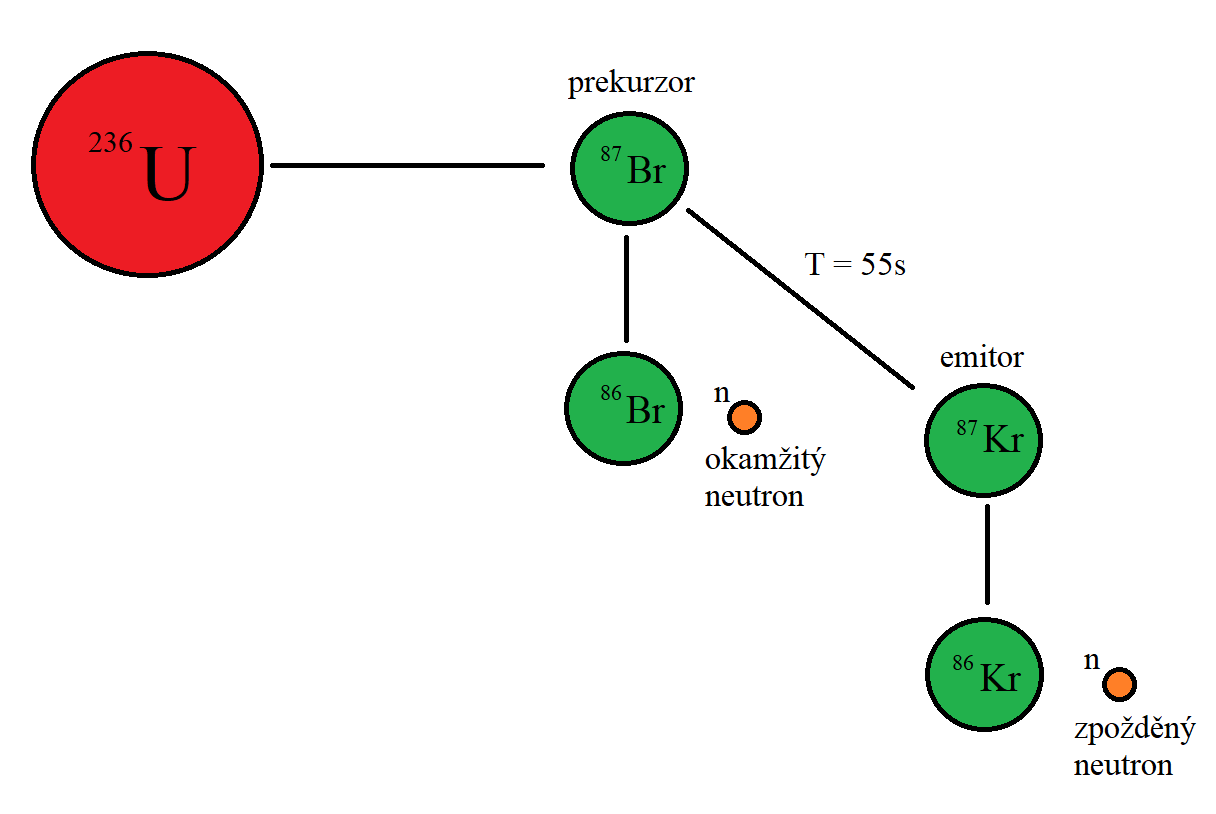
\includegraphics[width=0.8\textwidth]{img/1.png}
  \caption{Vznik okamžitých a zpožděných neutronů.}
  \label{fig_zpozdenky}
\end{figure}

Ačkoliv jsou zpožděné neutrony emitovány emitory, pro jejich charakteristiku je přiřazujeme původním prekurzorům. Těch mohou být desítky, proto je dělíme do několika skupin (JEFF 8~skupin, ENDF/B 6~skupin) podle poločasu rozpadu. Pro popis se zavádí tzv. \textbf{podíl zpožděných neutronů} $\beta$ (-) jako:

\begin{equation}
  \boxed{
  \beta \equiv \dfrac{\nu_D}{\nu_T},
  \label{zpozdenky}}
\end{equation}

kde:

\begin{itemize}
  \item $\nu_D$ (-) značí střední počet zpožděných neutronů vzniklých při jednom štěpení,
  \item $\nu_T$ (-) značí střední počet všech vzniklých neutronů.
\end{itemize}

Obdobně lze zavést $\nu_i$, $\beta_i$, $T_{1/2}^i$, $\tau_i$ a $\lambda_i$ pro jednotlivé skupiny (rodiny) zpožděných neutronů.\\

Dále se pro popis zavádí tzv. \textbf{efektivní střední doba života} $\ell^*$ (s) jako:

\begin{equation}
  \boxed{
  \ell^* \equiv \ell(1-\beta) + \sum_i \beta_i \tau_i,
  \label{efektivni_stredni_doba_zivota}}
\end{equation}

\textbf{efektivní střední doba vzniku} $\Lambda^*$ (s) jako:

\begin{equation}
  \boxed{
  \Lambda^* = \dfrac{\ell^*}{k_{\text{ef}}}
  \label{efektivni_stredni_doba_vzniku}}
\end{equation}

a \textbf{efektivní perioda reaktoru} $T_e^*$ (s) jako:

\begin{equation}
  \boxed{
  T_e^* \equiv \dfrac{\ell^*}{k_{\text{ef}} - 1}.
  \label{efektivni_perioda}}
\end{equation}

V podstatě se jedná o vážený průměr přes koeficienty $\beta$, a ačkoliv je podíl zpožděných neutronů minimální (do 1~\%), díky dlouhým $\tau$ se efektivní doba života velmi prodlouží a perioda reaktoru natáhne. Proto jsou zpožděné neutrony velmi důležité k řízení reaktoru. Nastane-li kritičnost na okamžitých neutronech, tento prodlužovací efekt zcela vymizí, perioda reaktoru se zkrátí až o několik řádů a máme tu druhý Černobyl.\\

\small

\textbf{Př. 2 -- perioda reaktoru podruhé:}

Pro klasický PWR reaktor platí, že $\sum \beta_i \tau_i \approx 0,1$~s. Vezměme hodnoty z př. 1 a koukněme se, jak se změní perioda reaktoru:

\begin{itemize}
  \item $k_{\text{ef}} = 1,01$ vychází efektivní perioda $T_e^* = 10$~s a za 1~s se změní výkon 1,105x (původně $2,69 \cdot 10^{43}$x),
  \item $k_{\text{ef}} = 1,001$ vychází efektivní perioda $T_e^* = 100$~s a za 1~s se změní výkon 1,010x (původně $2,20 \cdot 10^{4}$x),
  \item $k_{\text{ef}} = 1,0001$ vychází efektivní perioda $T_e^* = 1000$~s a za 1~s se změní výkon 1,001x (původně $2,72$x).
\end{itemize}

Je vidět, že s uvažováním zpožděných neutronů se efektivní perioda natáhne o několik řádů a reaktor už není tolik citlivý na změnu $k_{\text{ef}}$.\\

\normalsize

Lépe se řídí takové systémy, které mají větší $\beta$. Ve skutečnosti není reaktor takto ideální. Je třeba dále započítávat fotoneutrony (vznikající ($\gamma$,n) reakcí na lehkých jádrech, např. Be), více skupin zpožděných neutronů apod. Důležitá je i energetická závislost. Jelikož zpožděné neutrony vznikají s menší energií (0,5~MeV vs. 2~MeV) a mají náskok ve zpomalování. Díky nižší energii nemohou zpožděné neutrony nikdy zapříčinit štepení na štěpitelných jádrech.\\

Kvůli tomu všemu se zavádí tzv. \textbf{efektivní podíl zpožděných neutronů} $\beta_{\text{ef}}$ (-), což je umělá hodnota, která koriguje energetický rozdíl ve skupinách, jelikož každá ze skupin má jiný vliv na štepení. Lze ji zavést pomocí vztahu:

\begin{equation}
  \beta_{\text{ef}} = \beta \cdot I,
\end{equation}

kde $I$ (-) značí tzv. \textbf{funkci vlivu} a závisí na konkrétním reaktoru. Říká, jak je snadné pro zpožděné neutrony štěpit, oproti okamžitým neutronům. Obecně se pohybuje okolo $\approx 1$, při bližším studiu lze napsat: FR $<1$ a LWR $>1$.\\

Nyní si ještě ukažme rovnice jednobodové kinetiky se zpožděnými neutrony. Odvození je podobné jako v předcházejícím případě, pouze se původní vztah modifikuje. Výsledkem je soustava lineárních diferenciálních rovnic v destrukčním tvaru:

\begin{equation}
  \boxed{
  \dfrac{dN}{dt} = \dfrac{k_{\text{ef}}(1-\beta_{\text{ef}})-1}{\ell} N(t) + \sum_{i=1}^m \lambda_i C_i(t),
  \label{rovnice_kinetiky_zpozdenky_1}}
\end{equation}

\begin{equation}
  \boxed{
  \dfrac{dC_i}{dt} = -\lambda_i C_i(t) + \dfrac{\beta_{\text{ef},i} k_{\text{ef}} N(t)}{\ell},
  \label{rovnice_kinetiky_zpozdenky_2}}
\end{equation}

resp. rovnice v produkčním tvaru:

\begin{equation}
  \boxed{
  \dfrac{dN}{dt} = \dfrac{\rho - \beta_{\text{ef}}}{\Lambda} N(t) + \sum_{i=1}^m \lambda_i C_i(t),
  \label{rovnice_kinetiky_zpozdenky_3}}
\end{equation}

\begin{equation}
  \boxed{
  \dfrac{dC_i}{dt} = -\lambda_i C_i(t) + \dfrac{\beta_{\text{ef},i}  N(t)}{\Lambda}.
  \label{rovnice_kinetiky_zpozdenky_4}}
\end{equation}

\subsection{Přehled vzorečků}

Na závěr kapitolky rychlá vzorečkiáda (viz tabulka \ref{table_vzorecky_kinetika}).

\begin{table}[H]
\centering
\caption{Vzorečky s rovnicemi jednobodové kinetiky.}
\label{table_vzorecky_kinetika}
\begin{tabular}{@{}rcc@{}}
\toprule
\textbf{Parametr}                 & \textbf{Bez zpožděnek} & \textbf{Se zpožděnkami}   \\ \midrule
\textbf{Střední doba života}      & $\ell = \dfrac{1}{v \Sigma_a} \dfrac{1}{1+L^2B_g^2}$    & $\ell^* = \ell(1-\beta) + \sum_i \beta_i \tau_i$      \\ [15pt]
\textbf{Střední doba vzniku}      & $\Lambda = \dfrac{\ell}{k_{\text{ef}}}$                 & $\Lambda^* = \dfrac{\ell^*}{k_{\text{ef}}}$           \\ [15pt]
\textbf{Perioda reaktoru}         & $T_e = \dfrac{\ell}{k_{\text{ef}} - 1}$                 & $T_e^* = \dfrac{\ell^*}{k_{\text{ef}} - 1}$           \\ [15pt]
\textbf{R-ce v destrukčním tvaru} & $\dfrac{dN}{dt} = \dfrac{k_{\text{ef}} - 1}{\ell} N(t)$ & $\dfrac{dN}{dt} = \dfrac{k_{\text{ef}}(1-\beta_{\text{ef}})-1}{\ell} N(t) + \sum_{i=1}^m \lambda_i C_i(t)$        \\ [15pt]
                                  &                                                         & $\dfrac{dC_i}{dt} = -\lambda_i C_i(t)+\dfrac{\beta_{\text{ef},i} k_{\text{ef}} N(t)}{\ell}$           \\ [15pt]
\textbf{R-ce v produkčním tvaru}  & $\dfrac{dN}{dt} = \dfrac{\rho}{\Lambda} N(t)$           & $\dfrac{dN}{dt} = \dfrac{\rho - \beta_{\text{ef}}}{\Lambda} N(t) + \sum_{i=1}^m \lambda_i C_i(t)$                 \\ [15pt]
                                  &                                                         & $\dfrac{dC_i}{dt} = -\lambda_i C_i(t) + \dfrac{\beta_{\text{ef},i}  N(t)}{\Lambda}$                            \\ [15pt] \bottomrule
\end{tabular}
\end{table}
